\documentclass[11pt,a4paper]{article}

\usepackage[margin=1in]{geometry}
\usepackage{graphicx}
\usepackage{amsmath}

\title{Cellular Automata and Computational Universality}

\begin{document}

\maketitle

\begin{center}
    Thomas Archbold \\
    University of Warwick \\
    \texttt{T.Archbold@warwick.ac.uk}
\end{center}

\begin{abstract}
    Cellular automata are discrete models with the ability to not only give rise
    to beautiful, intricate patterns, but also to be used as powerful tools of
    computation, with applications in cryptography, error-correction coding, and
    simulation of computer processors, to name a few. They also raise profound
    questions about the nature of our reality, asking whether our universe could
    be one such automaton. This paper provides a discussion into these automata,
    exploring the various power and limitations of a number of specific rule
    sets, covering John Conway's well-known ``Game of Life'' to the more obscure
    ``Langton's ant'' and ``Wireworld''. In particular, it explores the notion
    of computational universality, or Turing completeness, an automaton's
    ability to simulate any conceivable computation, and considers their
    potential in the context of solving two specific problems, the Firing Squad
    Synchronization Problem and the Majority Problem. Existing solutions to
    these problems are explored, and their existing avenues for optimization are
    discussed. In order to fully appreciate the complex structures that can
    arise from such simple beginnings, this project also presents software to
    visualize and probe further into the nature of the automata highlighted.
\end{abstract}

\section{Introduction}
    A cellular automaton is a discrete model of computation which consists of a
    finite collection of ``cells'', each in one of a finite number of states.
    The state of each of these cells may evolve over the discrete progression of
    time in discrete steps, and may do so according to a deterministic set of
    rules specifying the state to which each cell is to progress, taking into
    account the states of cells in its neighbourhood. Their inherently discrete
    nature allows for strong analogies to be made with digital computers, and
    gifts them the ability to simulate digital processes and the potential to
    solve problems in this area. 
    
    Consider the cellular automaton defined by the simple rule:
    $$ a_{i}^{t+1} = a_{i-1}^{t} + a_{i+1}^{t} \mod{2} $$
    For any automaton, in each time step the rule is applied to all cells in the
    automaton instantaneously and simultaneously. In this case, our set of
    states is ${0,1}$, and for each cell we look at the cells immediately
    preceding and succeeding it: if exactly one of them is in state 1, then this
    cell will be in state 1 in the next time step. Otherwise it will be in state
    0.
    \begin{figure}[h]
        \begin{center}
            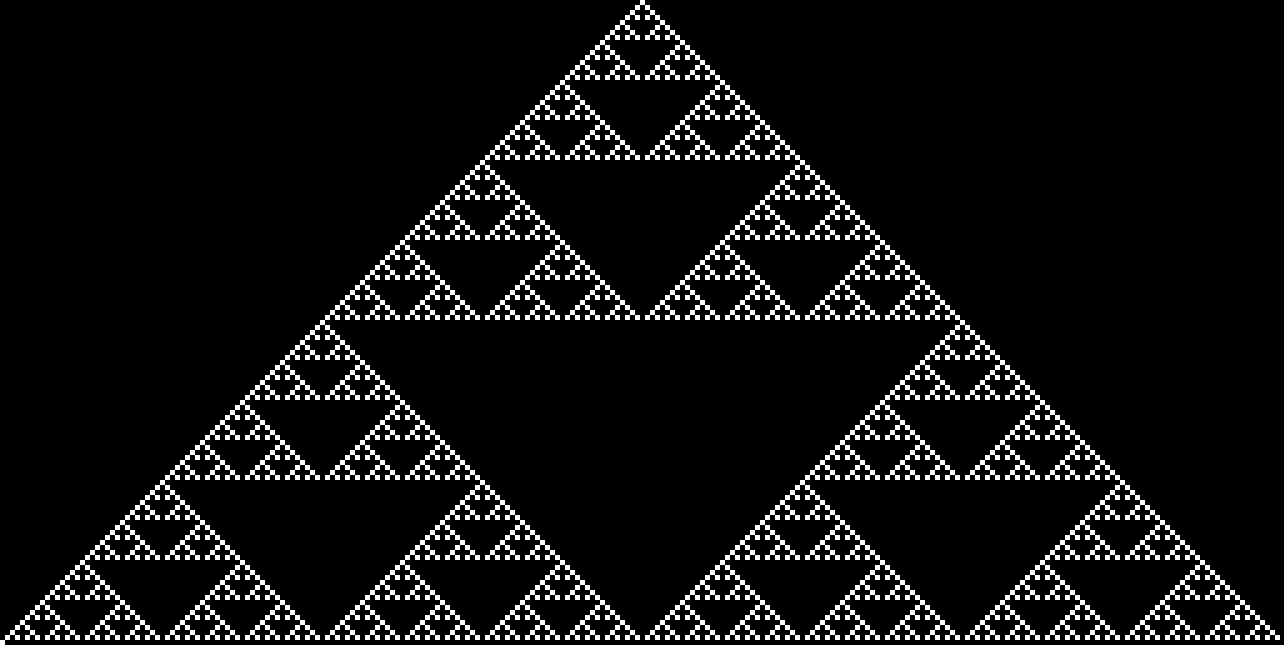
\includegraphics[width=10cm]{rule1.png}
            \caption{}
            \ref{}
        \end{center}
    \end{figure}
\section{}
\section{Examples}
\section{Applications}
\section{Computational Universality}
\section{Firing Squad Synchronization Problem}
\section{Majority Problem}
\section{}
\end{document}
